%% =====================================================================
%% Let It Crash, Then What?
%% A critical research proposal on Erlang/OTP as a runtime for
%% hierarchical Agent-to-Agent (A2A) systems.
%%
%% Overleaf: upload this single file and compile with pdfLaTeX
%% (the default). No .bib file is needed; the bibliography is inline.
%%
%% Drafted with AI assistance (Claude), November 2026. Web sources were
%% accessed on 18 Nov 2026. Verify every reference and every
%% version-specific claim again before submission.
%% Items printed in red are placeholders to complete.
%% =====================================================================
\documentclass[conference,letterpaper]{IEEEtran}
\IEEEoverridecommandlockouts

\usepackage[T1]{fontenc}
\renewcommand{\ttdefault}{lmtt}
\usepackage{textcomp}
\usepackage{cite}
\usepackage{amsmath,amssymb}
\usepackage{graphicx}
\usepackage{xcolor}
\usepackage{booktabs,tabularx,array}
\usepackage{listings}
\usepackage{tikz}
\usetikzlibrary{positioning,arrows.meta,fit,backgrounds,calc}
\usepackage{tcolorbox}
\usepackage{microtype}
\usepackage{xurl}
\usepackage[colorlinks=true,linkcolor=blue!50!black,citecolor=blue!50!black,
            urlcolor=blue!50!black]{hyperref}

\newcommand{\todo}[1]{\textcolor{red}{#1}}
\newcommand{\code}[1]{\texttt{#1}}
\newcommand{\gs}{\code{gen\_server}}
\newcommand{\gsm}{\code{gen\_statem}}
\newcolumntype{Y}{>{\raggedright\arraybackslash}X}
\newcolumntype{P}[1]{>{\raggedright\arraybackslash}p{#1}}
\emergencystretch=1.5em

\definecolor{kw}{RGB}{0,0,140}
\definecolor{cm}{RGB}{0,110,40}
\definecolor{str}{RGB}{150,20,20}
\lstdefinestyle{erl}{
  language=erlang,
  basicstyle=\ttfamily\footnotesize,
  keywordstyle=\bfseries\color{kw},
  commentstyle=\itshape\color{cm},
  stringstyle=\color{str},
  columns=fullflexible, keepspaces=true,
  frame=tb, framerule=0.4pt,
  aboveskip=4pt, belowskip=2pt,
  xleftmargin=0pt, xrightmargin=0pt,
  showstringspaces=false, captionpos=b,
  upquote=true
}
\lstset{style=erl}
\renewcommand{\lstlistingname}{Listing}

\hyphenation{Erlang Elixir super-vi-sor super-vi-sion orches-tra-tor}

\begin{document}

\title{Let It Crash, Then What? A Critical Research Proposal on Erlang/OTP
as a Runtime for Hierarchical Agent-to-Agent (A2A) Systems}

\author{\IEEEauthorblockN{\todo{[Author name --- to be completed]}}
\IEEEauthorblockA{School of Computing Science, Simon Fraser University\\
Burnaby, BC, Canada\\
\todo{[e-mail --- to be completed]}}}

\maketitle

\begin{abstract}
This research proposal examines whether Erlang, the BEAM virtual machine,
and the Open Telecom Platform (OTP) are a good substrate for hierarchies of
large language model (LLM) agents that interoperate through the
Agent2Agent (A2A) protocol, whose first stable specification (v1.0)
appeared in March 2026. The intuitive mapping is that agents become isolated
BEAM processes, teams become supervision trees in which supervisors restart
crashed agent workers, request-serving agents become \gs{} processes, and
agent lifecycles become \gsm{} machines. We test that intuition instead of
assuming it. A survey of existing work shows that the basic idea is not new:
Erlang multi-agent platforms with finite-state-machine behaviours existed by
2004, at least six BEAM frameworks already run LLM agents as supervised
processes, four Elixir libraries implement A2A, and actor-model agent
runtimes are mainstream on the JVM, .NET, and Python. We then argue against
the project. OTP supervision reacts to process exits, whereas the documented
failure modes of multi-agent LLM systems are specification, coordination,
and verification errors that never crash a process; naive restarts discard
expensive context and can repeat side effects; restart intensity silently
becomes a spending policy; distributed Erlang is a single trust domain that
cannot replace A2A across organizations; and runtime concurrency is rarely
the bottleneck. What survives is narrower and testable: automatic failure
detection, structured cancellation, protocol conformance by construction,
and the cost of recovery. We propose five research questions with
falsifiable, pre-registered hypotheses, a task-tree supervision
architecture, a fault-injection methodology with Python and BEAM baselines,
and explicit go/no-go gates. We expect, and will report, null results for
throughput.
\end{abstract}

\begin{IEEEkeywords}
Erlang/OTP, BEAM, actor model, multi-agent systems, LLM agents,
Agent2Agent protocol, supervision trees, fault tolerance, \gsm{},
durable execution
\end{IEEEkeywords}

%% =====================================================================
\section{Introduction}
%% =====================================================================

\IEEEPARstart{L}{arge} language model (LLM) agents are increasingly
composed rather than deployed alone: an orchestrating agent decomposes a
request, delegates subtasks to specialized agents, and integrates their
results~\cite{anthropic2025,adk-multi}. Composition across vendor and
organizational boundaries requires a wire protocol, and the Agent2Agent
(A2A) protocol has become the most visible candidate. Google announced it in
April 2025 and donated it to the Linux Foundation in June
2025~\cite{lf2025}; version~1.0, its first stable specification, followed in
March 2026~\cite{lf2026}, and in
August 2026 the project moved under the Linux Foundation's Agentic AI
Foundation alongside the Model Context Protocol~\cite{axios2026}.

The engineering problem behind A2A hierarchies looks familiar to anyone who
has built telecom software: many long-lived, concurrent, failure-prone
activities that must be isolated from one another, supervised, cancelled,
and observed. Erlang and OTP were designed for that class of
problem~\cite{armstrong2003,armstrong2007}. The research idea examined here
follows directly. Each agent is a BEAM process. Each team or delegation
subtree is an OTP supervision tree in which a supervisor restarts crashed
agent workers. Agents that serve other agents implement \gs, and an agent's
lifecycle is modelled with \gsm.

This proposal deliberately takes an adversarial stance towards its own
premise. An idea this intuitive tends to be rediscovered, and it has been:
the actor model was itself introduced as a formalism for artificial
intelligence~\cite{hewitt1973}, Erlang agent platforms predate LLMs by two
decades~\cite{distefano2003,fernandez2013}, and a crowded ecosystem of BEAM
agent frameworks now exists. Section~\ref{sec:survey} shows that
``agents as supervised processes'' is, in 2026, an implementation pattern
rather than a research contribution. Section~\ref{sec:critique} argues that
the pattern is also weaker than its advocates suggest, chiefly because the
failures that dominate LLM multi-agent systems are not the failures that OTP
supervision was designed to handle~\cite{cemri2025}.

\begin{tcolorbox}[colback=gray!6,colframe=gray!55,boxrule=0.5pt,arc=1pt,
  left=4pt,right=4pt,top=3pt,bottom=3pt,fontupper=\small]
\textbf{Verdict in brief.} The idea is sound engineering and weak research.
Running agents as supervised BEAM processes has been implemented many times,
and supervision as such does not address how LLM agents usually fail. The
project is worth doing only in the narrowed form proposed here: measure what
OTP adds to failure detection, cancellation, protocol conformance, and
recovery cost against strong non-BEAM baselines, and publish the result even
if it is null.
\end{tcolorbox}

The proposed research is accordingly narrower than the original idea, and it
makes four contributions. The first is a survey of existing solutions that
spans pre-LLM Erlang agent platforms, BEAM-native LLM agent frameworks, BEAM
implementations of A2A, and actor-based agent runtimes on other platforms
(Section~\ref{sec:survey} and Appendix~\ref{app:matrix}). The second is a
critical assessment that sets out thirteen reasons the project could fail or
produce no new knowledge (Section~\ref{sec:critique}). The third is a set of
five research questions with falsifiable hypotheses that isolate what the
BEAM could plausibly contribute (Section~\ref{sec:rq}). The fourth is a
reference architecture built on \emph{task-tree supervision} and a
fault-injection methodology with explicit criteria for pivoting or
abandoning the work
(Sections~\ref{sec:arch}--\ref{sec:gates}).

%% =====================================================================
\section{Background}\label{sec:background}
%% =====================================================================

\subsection{Erlang, the BEAM, and OTP}

Erlang programs consist of lightweight processes that share no memory and
communicate by asynchronous message passing, an instance of the actor
model~\cite{hewitt1973,agha1986,armstrong2003}. The BEAM
schedules processes preemptively and garbage-collects each process heap
independently, so a busy or memory-hungry process does not stall the others.
Processes can be \emph{linked}, so that an abnormal exit propagates as an
exit signal, or \emph{monitored}, so that an observer receives a message
when the target dies. OTP packages these primitives as
behaviours~\cite{cesarini2016}. A supervisor starts, monitors, and restarts
its children under a strategy (\code{one\_for\_one}, \code{one\_for\_all},
or \code{rest\_for\_one}), and each child declares whether it is
\code{permanent} (always restarted), \code{transient} (restarted only after
an abnormal exit), or \code{temporary} (never restarted)~\cite{otp-sup}. To
prevent restart loops, a supervisor has a maximum restart intensity: if more
than \code{intensity} restarts occur within \code{period} seconds, it
terminates its children and itself, escalating the failure to its own
supervisor. The defaults are one restart in five seconds~\cite{otp-sup}.
Children may also be marked \emph{significant}, so that a supervisor shuts
itself down automatically when they terminate~\cite{otp-sup}.

\gs{} implements the client--server pattern with synchronous calls, whose
default time-out is 5{,}000\,ms, and asynchronous casts~\cite{otp-genserver}.
\gsm{}, introduced in OTP~19 as the successor of \code{gen\_fsm}, adds
state-enter actions, state and event time-outs, and the ability to postpone
an event until the next state change~\cite{otp-statem}. The current major
release is OTP~29, published in May 2026~\cite{otp29}.

The ``let it crash'' philosophy rests on an empirical premise: many
production faults are transient ``Heisenbugs'' that disappear when the
computation is retried in a fresh state~\cite{gray1985}. Restarting a
fine-grained component is cheap only if process recovery is separated from
data recovery, so that the restart does not destroy durable
state~\cite{candea2004}. Both conditions matter for agents, as
Section~\ref{sec:critique} shows.

\subsection{LLM Agents and Hierarchical Multi-Agent Systems}

Operationally, an LLM agent is a loop. The model reads a context window and
emits either an answer or a tool invocation; the runtime executes the tool,
appends the result, and repeats until a stopping condition holds.
Multi-agent systems compose several such loops. The hierarchical form most
relevant here is orchestrator--worker. Anthropic's Research system uses a
lead agent that plans and spawns parallel subagents~\cite{anthropic2025},
and Google's Agent Development Kit (ADK) arranges agents in a parent and
sub-agent tree in which every agent has exactly one parent~\cite{adk-multi}.

The evidence on when such hierarchies help is mixed. Anthropic reports that
its multi-agent configuration outperformed a single agent by 90.2\% on an
internal research evaluation, that multi-agent systems use about fifteen
times as many tokens as chat, and that domains requiring shared context or
many inter-agent dependencies are a poor fit~\cite{anthropic2025}. A
controlled study of 180 agent configurations found that coordination helps
on parallelizable tasks but that, on sequential reasoning tasks, every
multi-agent variant tested degraded performance by 39--70\%~\cite{kim2025}.
Cognition argued in 2025 that multi-agent collaboration yields fragile
systems because decisions disperse and context is not
shared~\cite{yan2025}, and in 2026 narrowed rather than retracted that
position~\cite{yan2026}. Most important for this proposal, the MAST study of
more than 1{,}600 annotated traces from seven frameworks identifies fourteen
failure modes grouped into system design issues, inter-agent misalignment,
and task verification~\cite{cemri2025}.

\subsection{The A2A Protocol}

A2A targets communication between \emph{opaque} agents: agents that do not
share memory, tools, or internal state~\cite{a2a-spec,a2a-github}. A server
agent publishes an Agent Card that describes its skills, endpoints, and
security schemes. Version~1.0 specifies how cards are signed, using JSON Web
Signature over a payload canonicalized with the JSON Canonicalization Scheme,
and the project's own guidance stresses that a signature establishes the
card's integrity, not the trustworthiness of its publisher~\cite{aaif2026}.
Delegated work is represented as a Task whose status moves through
\code{SUBMITTED}, \code{WORKING}, \code{INPUT\_REQUIRED},
\code{AUTH\_REQUIRED}, \code{COMPLETED}, \code{FAILED}, \code{CANCELED}, and
\code{REJECTED} (plus a default \code{UNSPECIFIED}); the last four are
terminal, and the two \code{*\_REQUIRED} states are interruptions that wait
for the client~\cite{a2a-spec}. The abstract operations (among them
\code{SendMessage}, \code{SendStreamingMessage}, \code{GetTask},
\code{ListTasks}, \code{CancelTask}, and \code{SubscribeToTask}, plus
push-notification configuration and Agent Card retrieval) are bound to
JSON-RPC~2.0, gRPC, and HTTP+JSON, and clients state the protocol version
they speak in an \code{A2A-Version} header~\cite{a2a-spec}. Push
notifications are delivered at least once, so receivers must be idempotent,
and the project's own guidance describes the SDK's default in-memory task
store as unsuitable for production because tasks must survive
restarts~\cite{aaif2026}. Official SDKs exist for Python,
JavaScript/TypeScript, Java, Go, .NET, and Rust; there is none for Erlang or
Elixir~\cite{a2a-github}. A2A complements the Model Context Protocol (MCP),
which connects agents to tools and data rather than to other
agents~\cite{lf2026}.

\subsection{A Terminology Collision}

In LLM frameworks, ``supervisor'' usually names an orchestrating agent that
routes work to other agents. In OTP, a supervisor is a process that starts
and restarts children and, by design, contains no application
logic~\cite{otp-sup-princ}. These are different hierarchies with different
purposes. In this proposal ``supervisor'' always carries its OTP meaning,
and the LLM notion is called an \emph{orchestrator}.

%% =====================================================================
\section{Existing Solutions: Has This Been Done?}\label{sec:survey}
%% =====================================================================

We searched academic indexes, the Hex package registry, GitHub, vendor
documentation, and practitioner write-ups in November 2026. The search was
not systematic (making it so is work package WP0 in
Section~\ref{sec:method}), but it is sufficient to answer the question in
the section title. Appendix~\ref{app:matrix} summarizes the comparison.

\subsection{Erlang Agent Platforms Before LLMs}

Di Stefano and Santoro presented eXAT, the \emph{erlang eXperimental Agent
Tool}, in 2003 as an experiment in whether Erlang suits multi-agent
programming~\cite{distefano2003}. eXAT combined an Erlang rule engine for
agent reasoning, an execution environment in which agent behaviours were
object-oriented finite-state machines whose transitions could be triggered
by the agent's mental state, and FIPA-ACL messaging~\cite{distefano2004}; a
2005 paper compared Erlang with Java for agent engineering
explicitly~\cite{distefano2005}. Fern\'{a}ndez D\'{\i}az, Benac Earle, and
Fredlund later built eJason, an implementation of the BDI language Jason
that maps agents and agent-to-agent messages onto Erlang processes and
Erlang message passing~\cite{fernandez2013}, and extended it with
distribution and fault-tolerance constructs inspired by
Erlang~\cite{benacearle2017}. The idea of modelling agent behaviour as an
Erlang finite-state machine therefore predates \gsm{} itself, and the idea
of borrowing Erlang's distribution and fault tolerance for agents predates
LLM agents by a decade. What those platforms lacked, and what makes the
present question new at all, are agents whose reasoning is an expensive,
stochastic, external model call.

\subsection{BEAM-Native LLM Agent Frameworks}

The Elixir ecosystem now contains several frameworks that run LLM agents as
OTP processes. Jido~2.x represents an agent as an immutable data structure
updated by a pure command function; side effects are emitted as directives
that a \gs-based runtime executes, and the framework supports parent--child
agent hierarchies~\cite{jido} and hibernate/thaw persistence to pluggable
storage so that agents survive restarts~\cite{jido-storage}. Sagents, built
on the Elixir LangChain library~\cite{langchain-ex}, runs each agent as a
supervised \gs{} and adds human-in-the-loop interrupts, sub-agent
delegation, state persistence, and optional distribution across a cluster
with state migration~\cite{sagents,sagents-readme}. ExAgent states that each
agent \emph{is} a supervised process and offers message-passing
multi-agent sessions with durable persistence~\cite{exagent}. Condukt is
designed to integrate with OTP supervision trees~\cite{condukt}, and Lux
supervises agent processes in Elixir while delegating machine-learning work
to Python~\cite{lux}. Outside Elixir, Erlang ADK provides an agent
development kit in plain Erlang~\cite{erlang-adk}, and erlangchain provides
a dependency-free Erlang client for LLM APIs~\cite{erlangchain}. These
projects vary in maturity, and we found no peer-reviewed evaluation of any
of them; collectively, however, they already implement the ``supervisor
restarts crashed agent workers'' idea.

\subsection{A2A on the BEAM}

Four Elixir libraries implement A2A. The \code{a2a} package generates a
\gs{} per agent with task-lifecycle management, starts fleets of agents
under an \code{A2A.AgentSupervisor}, keeps tasks in ETS by default, accepts
protocol versions 0.3 and 1.0, and runs the official A2A Technology
Compatibility Kit (TCK); it is labelled pre-release and declares that it was
developed with significant AI assistance~\cite{a2a-actioncard}.
\code{a2a\_ex} concentrates on codecs and REST and JSON-RPC transports for
v0.3~\cite{a2a-ex}, \code{a2a\_elixir\_sdk} bridges an Elixir agent
development kit to A2A~\cite{a2a-elixir-sdk}, and \code{a2a\_engine}
separates the protocol contract from its transport precisely so that agents
in the same BEAM cluster need not pay for an HTTP/JSON round
trip~\cite{a2a-engine}. Carrying A2A semantics over native BEAM messaging
inside a cluster has therefore also been implemented, at least as library
design.

\subsection{Actor-Model Agent Runtimes on Other Platforms}

Outside the BEAM, the actor model is mainstream in agent infrastructure.
Microsoft rebuilt AutoGen in January 2025 around an actor model in which
agents exchange asynchronous messages~\cite{autogen2025}; its successor,
Microsoft Agent Framework, supports A2A and MCP~\cite{maf-sdtimes} and
reached version~1.0 in April 2026, with AutoGen moved to
maintenance~\cite{maf-vsm}. AgentScope introduced an actor-based
distribution framework in 2024, together with built-in fault-tolerance
mechanisms for erratic LLM and API behaviour~\cite{gao2024}. Akka launched
an agentic platform in July 2025~\cite{akka2025}. Its runtime provides actor
hierarchies in which parents supervise children with resume, restart, stop,
and escalate directives, as well as backoff
supervision~\cite{akka-capabilities}; yet its documentation has workflows,
not agents, decide which agents are needed, and Akka agents do not spawn
sub-agents~\cite{akka-patterns}. Dapr Agents runs agents on Dapr's workflow
engine, which is built on virtual actors and provides durable
execution~\cite{dapr-agents,dapr-docs}. Cloudflare's Agents SDK makes every
agent a Durable Object with its own persistent
state~\cite{cloudflare-agents}. The actor framing is therefore not a
differentiator, and several of these systems ship out of the box what OTP
does not: durable agent state and backoff.

\subsection{Graph Orchestration and Durable Execution}

LangGraph models an agent workflow as an explicit graph whose state a
checkpointer saves after each step, so that execution can resume from the
last successful checkpoint after a failure~\cite{langgraph-durable}. A
vendor critique notes that checkpointing alone neither detects a crashed
worker nor prevents two workers from resuming the same
thread~\cite{diagrid2025}, which is exactly the gap that OTP links and
monitors fill. This complementarity, rather than any claim of superiority,
is the most promising entry point for research on the BEAM
(Section~\ref{sec:survives}).

\subsection{Verdict: What Exists and What Does Not}\label{sec:gaps}

Has the idea already been implemented? In its basic form, yes, and
repeatedly: agents as supervised BEAM processes, A2A on the BEAM including
in-cluster transport, finite-state-machine agent behaviours on Erlang, and
actor-model agent runtimes with supervision at industrial scale. We did
\emph{not}, however, find three things. The first is a peer-reviewed empirical
comparison of OTP supervision with durable-execution and actor alternatives
under a fault model specific to LLM agents. The second is a \gsm{} encoding
of the A2A~v1.0 task lifecycle validated against the official TCK and
adversarial peers. The third is any quantification of what restart policies
cost in tokens, money, and duplicated side effects. These gaps are modest.
They are worth closing only if the results are reported whether or not they
favour the BEAM.

%% =====================================================================
\section{Critical Assessment: Why This Project May Fail}\label{sec:critique}
%% =====================================================================

This section argues against the proposal as forcefully as we can. Each
subsection states a weakness and explains why it matters; mitigations, where
they exist, are folded into Sections~\ref{sec:rq}--\ref{sec:method}.

\subsection{C1: The Novelty Is Thin}

Mapping agents to processes, teams to supervision trees, and lifecycles to
state machines is the first design an Erlang programmer would sketch, and
Section~\ref{sec:survey} shows that many already have. A project that builds
yet another BEAM agent framework and demonstrates that a crashed worker is
restarted would be an engineering report, not research. Any contribution
must come from measurement and from the specific gaps identified in
Section~\ref{sec:gaps}.

\subsection{C2: Supervision Addresses the Wrong Failures}

OTP supervision is triggered by process exits. None of the fourteen failure
modes in MAST is a process crash; all three of its categories (system design
issues, inter-agent misalignment, and task verification) describe agents
that keep running while doing the wrong thing~\cite{cemri2025}. An agent
that fabricates a citation, ignores another agent's input, repeats steps, or
declares a task complete prematurely returns \code{\{ok, Result\}}; no exit
signal is emitted and no supervisor acts. Even when a failure can be turned
into a crash, restarting is a meaningful remedy only for transient
faults~\cite{gray1985}. Re-running an LLM agent on the same specification
resamples a stochastic model, which may succeed by chance but does not
repair the cause. Supervision trees solve the class of agent failures that
look like telecom failures, and the available evidence suggests that this
is not where multi-agent systems mostly fail.

\subsection{C3: Restarting Throws Away the Expensive Part}

OTP restarts a child from its start function, that is, from its initial
state. For an agent in the middle of a task, the valuable state is the
accumulated context: the plan, intermediate results, and tool outputs that
cost tokens and minutes to produce. Microreboots are cheap because process
recovery is separated from data recovery~\cite{candea2004}; OTP provides only
the former. Anthropic reports that agents are stateful and errors compound,
that restarting from the beginning is too expensive, and that it therefore
built resumption from the point of failure, combined with retries and
regular checkpoints~\cite{anthropic2025}. The A2A builder guidance likewise
rejects in-memory task stores for production~\cite{aaif2026}. A credible
BEAM design therefore needs checkpointing and replay, that is, durable
execution, which LangGraph, Dapr, Cloudflare Durable Objects, and Jido's
hibernate/thaw already
provide~\cite{langgraph-durable,dapr-docs,cloudflare-agents,jido-storage}.
If the project ends up re-implementing durable execution in Erlang, it must
show what OTP adds, or it has merely ported an existing idea.

\subsection{C4: Restarts Can Duplicate Side Effects}

Agents act through tools, and many tools are not idempotent: they send
messages, write records, place orders, or delegate to other agents. If an
agent crashes after a tool call has taken effect but before the result is
recorded, a restart repeats the call. A2A itself delivers push notifications
at least once and expects receivers to be idempotent~\cite{aaif2026}. OTP
offers no effect journal, idempotency keys, or compensation; these must be
designed. This is the most dangerous property of naive ``let it crash'' for
agents, and it is a safety argument, not a performance one.

\subsection{C5: Restart Intensity Becomes a Spending Policy}

OTP's restart intensity counts restarts per unit of time, and the default
tolerates one restart in five seconds~\cite{otp-sup}. For an LLM agent,
every restart that replays work spends tokens, so restart intensity is in
effect an unbudgeted spending limit. Failures are also correlated: a
provider outage or a rate-limit response hits every sibling that uses the
same model at once, which under \code{one\_for\_all} or
\code{rest\_for\_one} multiplies restarts and quickly escalates a local fault
into the loss of an entire subtree. The standard supervisor restarts
immediately and has no built-in backoff, whereas Akka offers backoff
supervision as a platform feature~\cite{akka-capabilities}; circuit breaking
and backoff must be added. A supervision tree tuned for telecom workloads,
where restarts are fast, cheap, and independent, is mistuned for agents,
where they are slow, expensive, and correlated.

\subsection{C6: The Runtime Is Rarely the Bottleneck}

It is often argued that because the BEAM can run very large numbers of
processes (the default limit is 1{,}048{,}576~\cite{otp-limits}), it scales
agent systems. The premise is true and the inference is weak. An agent
spends most of its life waiting for a model response that takes seconds,
costs money, and is subject to provider rate limits; the binding constraints
are inference latency, token budgets, and quotas~\cite{anthropic2025}.
Event-loop runtimes routinely hold thousands of concurrent outstanding HTTP
requests, so for I/O-bound agents the BEAM's concurrency advantage is
unlikely to be visible in end-to-end latency or throughput. We expect the
corresponding hypothesis (H2c) to yield a null result and will report it as
such.

\subsection{C7: Distributed Erlang Is a Single Trust Domain}

A2A exists to connect agents across organizational boundaries. Distributed
Erlang assumes the opposite. Its documentation warns that starting a
distributed node without TLS distribution exposes it to attacks that may
give an attacker complete access to the node and, by extension, the
cluster~\cite{otp-dist}. The magic cookie is protection against accidental
connections rather than a cryptographic mechanism, inter-node traffic is
clear text by default, and any connected node can spawn processes on any
other~\cite{otp-dist}. Even TLS distribution has had authorization flaws:
CVE-2026-48860, fixed in OTP~29.0.2, let any holder of a CA-signed
certificate bypass the LAN allow-list of \code{inet\_tls\_dist} and obtain
full distribution access~\cite{cve2026-48860,otp2902}. Distributed Erlang
can therefore only ever be an intra-organization optimization behind an A2A
gateway; it cannot replace A2A at a trust boundary. Its scalability is also
bounded. The RELEASE project documented limits caused by the default fully
connected topology and global name registration~\cite{trinder2017}, and
Partisan reports up to an order of magnitude more nodes, along with large
throughput and latency gains, by replacing the default distribution
layer~\cite{meiklejohn2019}. Neither result suggests that the stock layer is
the right substrate for large agent populations.

\subsection{C8: BEAM Isolation Is Not a Sandbox}

Process isolation on the BEAM is fault isolation, not security isolation.
Every process on a node runs with the node's operating-system privileges and
can call any loaded module, including those that open ports or run shell
commands. An agent that executes model-generated code, or whose tools can be
steered by prompt injection or poisoned Agent Cards~\cite{habler2025,
aaif2026}, is not confined by being an Erlang process; operating-system or
WebAssembly sandboxing is still required. Two BEAM-specific hazards stand
out. Atoms are not garbage-collected and are limited to 1{,}048{,}576 by
default~\cite{otp-eff,otp-limits}, so any code path that turns untrusted A2A payload
keys or Agent Card fields into atoms lets a remote peer exhaust the table
and crash the node. Native implemented functions (NIFs), used by numerical
and some JSON libraries, run inside the VM, and a crashing NIF takes down
the whole node~\cite{otp-nif}, bypassing supervision entirely. The
platform's own attack surface is also real: CVE-2025-32433, a CVSS~10.0
pre-authentication remote-code-execution flaw in OTP's SSH server, was
disclosed in April 2025~\cite{cve2025-32433} and later added to CISA's
catalogue of known exploited vulnerabilities~\cite{cve2025-32433-kev}.

\subsection{C9: Supervision Hierarchy Is Not Delegation Hierarchy}\label{sec:conflation}

The original idea conflates two hierarchies. A supervision tree is a
failure-management structure whose supervisors contain no business logic
and exist only to start, stop, and restart children~\cite{otp-sup-princ}. A
delegation hierarchy is semantic and dynamic: an orchestrator decides at run
time which agents to involve, agents may call peers, and the agent graph may
contain cycles. An orchestrating agent is therefore an OTP \emph{worker},
not an OTP supervisor. Furthermore, an A2A peer owned by another
organization cannot be placed under a local supervisor at all; one can only
supervise the local process that represents the remote task. Industrial
designs make the same separation: Akka lets workflows, not agents, decide
which agents are needed~\cite{akka-patterns}. Section~\ref{sec:arch} turns
this criticism into a design principle by supervising the \emph{task} tree
rather than the agent graph.

\subsection{C10: A \gs{} per Agent Is a Serialization Point}

A \gs{} processes one message at a time. An agent that serves other agents
and calls a model inline blocks every other caller for the duration of a
model call, which commonly takes seconds. The default 5{,}000\,ms
\code{gen\_server:call} time-out~\cite{otp-genserver} is shorter than many
model calls, so naive designs produce spurious time-outs, which crash
callers, which trigger restarts. Synchronous mutual calls (agent~A calls~B
while~B, to answer, calls~A) deadlock until the time-out fires, a classic
Erlang pitfall that becomes likely in cyclic agent graphs. The remedies are
well known: deferred replies with \code{gen\_server:reply/2}, asynchronous
requests with \code{send\_request/2} and \code{receive\_response/2}, and
worker pools (Listing~\ref{lst:async}). Once they are applied, however,
``an agent implements \gs'' becomes an implementation detail rather than a
model of agency.

\subsection{C11: \gsm{} Models the Protocol, Not the Agent}

The A2A task lifecycle has eight meaningful states and a small set of legal
transitions. Encoding it in \gsm{} is straightforward and, as eXAT shows,
not new in spirit~\cite{distefano2004}. The decisions that matter (what to
ask, which tool to call, when the task is done) are made inside the model
and are invisible to the state machine. \gsm{} nonetheless adds modest but
real value: illegal transitions are rejected by construction,
\code{INPUT\_REQUIRED} can carry a state time-out, and messages that arrive
in the wrong state can be postponed rather than lost. Whether this reduces
protocol violations relative to existing implementations is an empirical
question (RQ1).

\subsection{C12: Ecosystem, Evaluation, and Venue Risk}

There is no official A2A SDK for the BEAM~\cite{a2a-github}; the community
libraries are young, and the most complete one is labelled
pre-release~\cite{a2a-actioncard}. LLM providers' official SDKs target other
languages, so a BEAM implementation depends on community clients or bespoke
HTTP code. LLM behaviour is nondeterministic and models are versioned and
retired on vendor schedules, which threatens reproducibility; experiments
with hosted models cost money, which limits sample sizes. The investigator's
fluency in Erlang creates implementer bias against the Python baselines.
Finally, the work falls between communities: AI venues may not value
runtime engineering, and programming-language venues may not value LLM
evaluation.

\subsection{C13: The Premise Itself Is Contested}

Deep A2A hierarchies are not obviously desirable. Multi-agent systems
consume an order of magnitude more tokens than chat~\cite{anthropic2025},
degrade sequential tasks in controlled experiments~\cite{kim2025}, and
remain contested among practitioners~\cite{yan2025,yan2026}. A runtime
optimized for deep hierarchies may be optimizing a pattern the field is
narrowing. The proposal therefore evaluates shallow hierarchies (depth two
to three) on parallelizable workloads, where the evidence favours
multi-agent designs, and makes no claim that deeper is better.

\subsection{What Survives the Critique}\label{sec:survives}

Four properties survive and define the research. First, failure detection
is automatic and immediate: links and monitors report a dead process without
polling, which is precisely what checkpoint-only orchestration
lacks~\cite{diagrid2025}. Second, cancellation can be structured:
terminating a supervisor terminates its subtree, so an A2A \code{CancelTask}
can stop all descendant work, and the token spending it entails, instead of
relying on cooperative cancellation in every agent. Third, scheduling is
preemptive and heaps are per process, so a runaway agent loop cannot starve
its siblings the way a CPU-bound coroutine can stall a single-threaded event
loop. Fourth, the platform is unusually observable and upgradable in place.
This matters because long-running agents make ordinary deployments
disruptive enough that Anthropic resorted to rainbow
deployments~\cite{anthropic2025}; whether hot upgrades of stateful agent
processes are practical is itself an open question. Our working hypothesis
is that the BEAM's advantages for A2A hierarchies lie in containment,
detection, cancellation, and operability, not in throughput and not in
semantic reliability.

%% =====================================================================
\section{Research Questions and Hypotheses}\label{sec:rq}
%% =====================================================================

Each question is paired with hypotheses and the observations that would
falsify them. Hypotheses, metrics, and analysis code will be registered
before data collection (Section~\ref{sec:stats}).

\textbf{RQ1 (Conformance by construction).} Can the A2A~v1.0 task lifecycle
be encoded as a \gsm{} so that the implementation passes the mandatory
categories of the official TCK, and does the encoding reduce protocol
violations when peers misbehave? \emph{H1:} a \gsm-based server passes all
mandatory TCK categories and, under grammar-based fuzzing of message
sequences, never performs an illegal state transition, whereas at least one
comparison implementation does. H1 is falsified if the encoding fails
mandatory TCK tests after the time-boxed effort, or if no comparison
implementation exhibits violations, in which case the encoding offers no
measurable benefit. Runtime monitoring of Erlang actors against multiparty
session types~\cite{fowler2016,fowler2026} provides the formal backdrop for
the conformance monitor used here.

\textbf{RQ2 (Recovery under an LLM fault model).} Under the fault model of
Section~\ref{sec:faults}, how do recovery outcomes compare among four
configurations: (B0) naive OTP restart from the initial state; (B1) OTP
supervision combined with checkpointing and an effect journal; (B2)
LangGraph with a persistent checkpointer; and (B3) a durable-execution agent
runtime? \emph{H2a:} B0 wastes more tokens and duplicates more side effects
than every other configuration; this is a sanity check that naive ``let it
crash'' is harmful. \emph{H2b:} B1 is non-inferior to B3 in task completion
and duplicated effects, within margins fixed in advance, while detecting
process failures faster than B2. \emph{H2c:} differences in end-to-end
latency and throughput among B1--B3 lie within the run-to-run variance
caused by model latency. H2b is falsified if B1 is inferior on either
outcome; H2c is falsified if the BEAM configuration is significantly faster
end to end, which would itself be a notable finding.

\textbf{RQ3 (Semantic supervision and budget-aware restarts).} Does turning
detectable semantic failures into crashes, through output-schema validation,
loop detection, budget monitors, and verifier models, and then restarting
from the last checkpoint improve successful tasks per unit of cost? And does
denominating restart intensity in tokens or money rather than in restart
counts prevent runaway spending? \emph{H3a:} semantic fail-fast improves
success per dollar for format and loop failures but not for failures that
originate in the task specification (MAST's system-design category).
\emph{H3b:} a token-denominated restart budget bounds worst-case spending
under correlated provider failures without reducing success under
independent failures.

\textbf{RQ4 (Structured cancellation).} When a client cancels the root task
of a delegation hierarchy, how much work continues afterwards? \emph{H4:}
with cancellation propagated through task subtrees, tokens consumed after
\code{CancelTask} in hierarchies of depth three fall, relative to
cooperative cancellation in the Python baselines, by at least a
pre-specified margin (provisionally 50\%). A smaller or non-significant
reduction falsifies H4.

\textbf{RQ5 (Placing the trust boundary).} What does it cost to keep
distributed Erlang strictly inside one trust domain, with A2A over HTTPS at
every boundary? \emph{H5:} native in-cluster delivery reduces per-message
overhead relative to JSON-RPC over HTTP by at least an order of magnitude,
but the saving is below 2\% of end-to-end task latency, so it is not, by
itself, a reason to choose the BEAM.

%% =====================================================================
\section{Proposed Architecture}\label{sec:arch}
%% =====================================================================

\begin{figure*}[t]
\centering
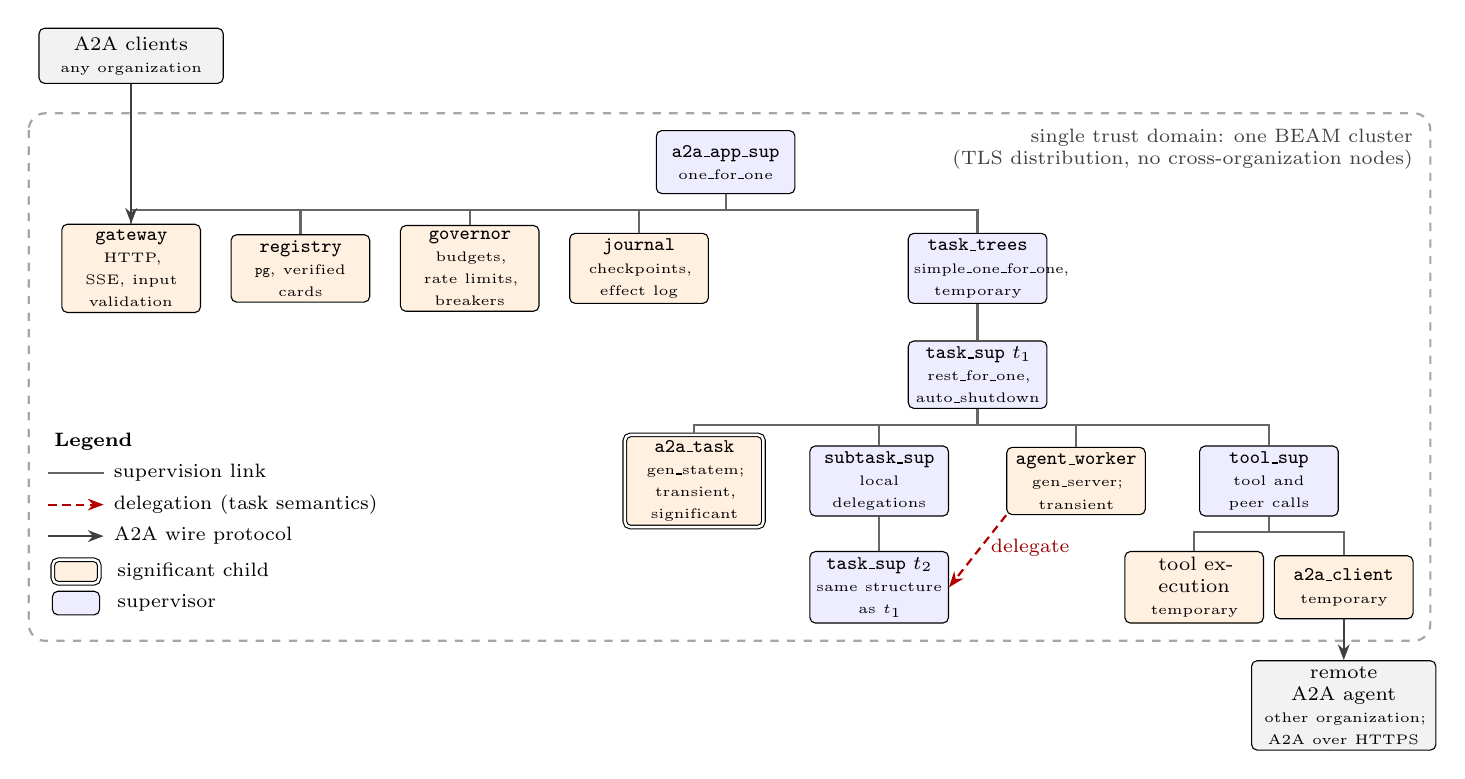
\begin{tikzpicture}[
  font=\scriptsize,
  sup/.style={draw, rounded corners=2pt, fill=blue!7, align=center,
    text width=1.62cm, minimum height=0.8cm, inner sep=2pt},
  wrk/.style={draw, rounded corners=2pt, fill=orange!12, align=center,
    text width=1.62cm, minimum height=0.8cm, inner sep=2pt},
  sig/.style={wrk, double, double distance=0.9pt},
  ext/.style={draw, rounded corners=2pt, fill=gray!10, align=center,
    text width=2.2cm, minimum height=0.7cm, inner sep=2pt},
  link/.style={thick, black!60},
  deleg/.style={-{Stealth[length=2mm]}, densely dashed, thick,
    red!70!black},
  wire/.style={-{Stealth[length=2mm]}, thick, black!75}
]
% ---- external parties -------------------------------------------------
\node[ext] (clients) at (-7.55,1.35) {A2A clients\\{\tiny any organization}};
\node[ext] (remote)  at (7.85,-6.9) {remote A2A agent\\{\tiny other organization; A2A over HTTPS}};
% ---- level 0 ----------------------------------------------------------
\node[sup] (app) at (0,0) {\code{a2a\_app\_sup}\\{\tiny one\_for\_one}};
% ---- level 1: services and task trees ---------------------------------
\node[wrk] (gw)  at (-7.55,-1.35) {\code{gateway}\\{\tiny HTTP, SSE, input validation}};
\node[wrk] (reg) at (-5.4,-1.35)  {\code{registry}\\{\tiny \code{pg}, verified cards}};
\node[wrk] (gov) at (-3.25,-1.35) {\code{governor}\\{\tiny budgets, rate limits, breakers}};
\node[wrk] (jnl) at (-1.1,-1.35)  {\code{journal}\\{\tiny checkpoints, effect log}};
\node[sup] (tt)  at (3.2,-1.35)   {\code{task\_trees}\\{\tiny simple\_one\_for\_one, temporary}};
% ---- level 2: one task subtree ----------------------------------------
\node[sup] (t1) at (3.2,-2.7) {\code{task\_sup} $t_1$\\{\tiny rest\_for\_one, auto\_shutdown}};
% ---- level 3: children of t1, in start order --------------------------
\node[sig] (fsm) at (-0.4,-4.05) {\code{a2a\_task}\\{\tiny gen\_statem; transient, significant}};
\node[sup] (sub) at (1.95,-4.05) {\code{subtask\_sup}\\{\tiny local delegations}};
\node[wrk] (ag)  at (4.45,-4.05) {\code{agent\_worker}\\{\tiny gen\_server; transient}};
\node[sup] (tl)  at (6.9,-4.05)  {\code{tool\_sup}\\{\tiny tool and peer calls}};
% ---- level 4 ----------------------------------------------------------
\node[sup] (t2)  at (1.95,-5.4) {\code{task\_sup} $t_2$\\{\tiny same structure as $t_1$}};
\node[wrk] (tool) at (5.95,-5.4) {tool execution\\{\tiny temporary}};
\node[wrk] (acl)  at (7.85,-5.4) {\code{a2a\_client}\\{\tiny temporary}};
% ---- trust boundary ---------------------------------------------------
\begin{scope}[on background layer]
  \draw[dashed, rounded corners=6pt, gray!70, thick]
    (-8.85,0.62) rectangle (8.95,-6.08);
\end{scope}
\node[anchor=north east, text=gray!50!black, align=right]
  at (8.85,0.55) {single trust domain: one BEAM cluster\\
  (TLS distribution, no cross-organization nodes)};
% ---- supervision edges (buses) ----------------------------------------
\draw[link] (app.south) -- ++(0,-0.2) coordinate (b0);
\foreach \n in {gw,reg,gov,jnl,tt} \draw[link] (b0) -| (\n.north);
\draw[link] (tt.south) -- (t1.north);
\draw[link] (t1.south) -- ++(0,-0.2) coordinate (b1);
\foreach \n in {fsm,sub,ag,tl} \draw[link] (b1) -| (\n.north);
\draw[link] (sub.south) -- (t2.north);
\draw[link] (tl.south) -- ++(0,-0.2) coordinate (b2);
\foreach \n in {tool,acl} \draw[link] (b2) -| (\n.north);
% ---- delegation and wire edges ----------------------------------------
\draw[deleg] (ag.south west) -- node[right, text=red!60!black, pos=0.45]
  {delegate} (t2.east);
\draw[wire] (clients.south) -- (gw.north);
\draw[wire] (acl.south) -- (remote.north);
% ---- legend -----------------------------------------------------------
\node[anchor=west] at (-8.65,-3.55) {\textbf{Legend}};
\draw[link] (-8.6,-3.95) -- ++(0.7,0) node[right, text=black] {supervision link};
\draw[deleg] (-8.6,-4.35) -- ++(0.7,0) node[right, text=black] {delegation (task semantics)};
\draw[wire] (-8.6,-4.75) -- ++(0.7,0) node[right, text=black] {A2A wire protocol};
\node[sig, text width=0.45cm, minimum height=0.3cm] at (-8.25,-5.2) {};
\node[anchor=west] at (-7.85,-5.2) {significant child};
\node[draw, rounded corners=2pt, fill=blue!7, minimum width=0.6cm,
  minimum height=0.3cm] at (-8.25,-5.6) {};
\node[anchor=west] at (-7.85,-5.6) {supervisor};
\end{tikzpicture}
\caption{Reference architecture based on task-tree supervision. Supervision
mirrors the tree of A2A \emph{tasks}, which is a tree by construction
because each task has exactly one requester, rather than the graph of
\emph{agents}, which may contain cycles. Children of \code{task\_sup} are
listed in start order, which \code{rest\_for\_one} turns into a dependency
order. A delegating agent starts the child task under \code{subtask\_sup} and
monitors it, so locally delegated subtasks nest under the delegating task
and finishing or cancelling $t_1$ shuts down $t_2$. Remote peers are never
supervised, only the local \code{a2a\_client} that represents them.
Distributed Erlang never crosses the outer boundary.}
\label{fig:arch}
\end{figure*}

Figure~\ref{fig:arch} shows the reference design. It keeps apart the three
structures that Section~\ref{sec:conflation} warns against conflating: the
supervision tree (solid lines), the delegation relation (dashed arrows), and
the trust boundary (outer box).

\subsection{Task-Tree Supervision}

The central design decision is to make supervision mirror the tree of A2A
tasks rather than the graph of agents. Agents may delegate to one another in
cycles, but every A2A task is created by exactly one request from exactly
one client, so tasks and their subtasks always form a tree. Each task is
represented by a \code{task\_sup} subtree with four children in start order
(Listing~\ref{lst:sup}). The first is the \code{a2a\_task} \gsm{}
(Listing~\ref{lst:fsm}, Fig.~\ref{fig:fsm}), which owns the protocol
lifecycle and journals every transition before acting on it. The second is
\code{subtask\_sup}, under which locally delegated subtasks are started as
nested \code{task\_sup} subtrees. The third is \code{agent\_worker}, a \gs{}
that runs the model loop and, after a restart, resumes from the latest
checkpoint rather than from its initial state. The fourth is
\code{tool\_sup}, whose children (tool executions and \code{a2a\_client}
processes that stand for remote peers) are \code{temporary} and are never
restarted automatically; a failed tool call is reported to the agent and
retried only if the effect journal shows that the action did not complete
or the tool is declared idempotent.

Under \code{rest\_for\_one}, start order becomes dependency order. If the
lifecycle machine fails, everything after it restarts. If the agent fails,
its in-flight tool calls are terminated with it, but the lifecycle and the
subtasks it is coordinating survive, and the resumed agent reattaches to them
through the journal. If a tool fails, nothing restarts. Because
\code{a2a\_task} is a significant, transient child and \code{task\_sup} uses
\code{auto\_shutdown}~\cite{otp-sup}, a task that reaches a terminal state
stops normally, and its entire subtree, including nested subtasks, shuts
down with it. Each \code{a2a\_client} traps exits so that its
\code{terminate/2} callback can send a best-effort \code{CancelTask} to the
remote peer. This is the structured cancellation that RQ4 measures.

One subtlety shapes the design. When a task subtree exhausts its restart
intensity, its supervisor terminates the children with reason
\code{shutdown}, which a child cannot distinguish from a shutdown caused by
the cancellation of an ancestor task. The design therefore never infers a
protocol outcome inside a dying process. Cancellation is journaled top-down
before any shutdown begins: the cancelling machine records
\code{CANCELED} for its live descendants and then stops. The gateway
reports any task that has neither a live lifecycle machine nor a terminal
journal record as \code{FAILED}. Supervision shutdown reclaims processes and
stops in-flight work; the journal records outcomes.

\begin{lstlisting}[float=t, caption={Per-task supervisor. Start order
encodes dependency; the significant lifecycle child triggers automatic
shutdown of the whole task subtree.}, label={lst:sup}]
init(Task) ->
  Flags = #{strategy => rest_for_one,
            intensity => 3, period => 60,
            auto_shutdown => any_significant},
  Kids =
   [#{id => fsm, restart => transient,
      significant => true,
      start => {a2a_task, start_link, [Task]}},
    #{id => subtasks, type => supervisor,
      start => {subtask_sup, start_link, []}},
    #{id => agent, restart => transient,
      start => {agent_worker, start_link,
                [Task]}},
    #{id => tools, type => supervisor,
      start => {tool_sup, start_link, []}}],
  {ok, {Flags, Kids}}.
\end{lstlisting}

\begin{lstlisting}[float=t, caption={Core of the A2A task lifecycle as a
\gsm{} (\code{auth\_required} clauses are analogous and elided).},
label={lst:fsm}]
-module(a2a_task).
-behaviour(gen_statem).
-export([start_link/1, init/1, callback_mode/0,
         handle_event/4]).
-define(INPUT_TTL, timer:minutes(30)).

start_link(T) ->
    gen_statem:start_link(?MODULE, T, []).
init(T) -> {ok, submitted, T}.
callback_mode() ->
    [handle_event_function, state_enter].

%% Journal every transition before acting on it.
handle_event(enter, _Old, input_required, T) ->
    journal(T, input_required),
    {keep_state_and_data,
     [{state_timeout, ?INPUT_TTL, expired}]};
handle_event(enter, _Old, S, T) ->
    journal(T, S), keep_state_and_data;
%% CancelTask is legal in every live state.
handle_event({call, From}, cancel, _S, T) ->
    cancel_descendants(T),
    finish(T, canceled, [{reply, From, ok}]);
handle_event(cast, accept, submitted, T) ->
    {next_state, working, T};
handle_event(cast, reject, submitted, T) ->
    finish(T, rejected, []);
handle_event(info, {need_input, Q}, working, T) ->
    {next_state, input_required, T#{q => Q}};
handle_event(info, {done, Art}, working, T) ->
    finish(T#{artifacts => Art}, completed, []);
handle_event(info, {error, Why}, working, T) ->
    finish(T#{error => Why}, failed, []);
handle_event(cast, {msg, _}, working, _T) ->
    {keep_state_and_data, [postpone]};
handle_event(cast, {msg, M}, input_required, T) ->
    resume_agent(T, M),
    {next_state, working, T};
handle_event(state_timeout, expired,
             input_required, T) ->
    finish(T, failed, []).
%% Other events: function_clause, i.e. a crash.

finish(T, Final, Replies) ->
    journal(T, Final),
    {stop_and_reply, normal, Replies, T}.
%% journal/2, resume_agent/2, and
%% cancel_descendants/1 elided.
\end{lstlisting}

\subsection{The Lifecycle Machine}

Listing~\ref{lst:fsm} encodes the lifecycle of Fig.~\ref{fig:fsm} with
\code{handle\_event\_function} and state-enter calls. Three \gsm{} features
do real work. State-enter calls journal every transition in one place, so
the journal is the resume point after any crash. A single clause makes
\code{CancelTask} legal in every live state. Postponement holds a follow-up
message that arrives while the agent is working until the machine next
changes state, instead of dropping it or interleaving it with the running
model call. Terminal states are not machine states at all: the process
journals the outcome and stops normally, which triggers the subtree shutdown
described above. Unmatched events raise \code{function\_clause}, which turns
local protocol violations into crashes that the supervisor handles. This is
deliberate for events produced inside the task subtree, but it would be a
denial-of-service vector if events from untrusted peers reached the machine
unvalidated; the gateway therefore validates every inbound message against
the protocol schema first.

\begin{figure}[t]
\centering
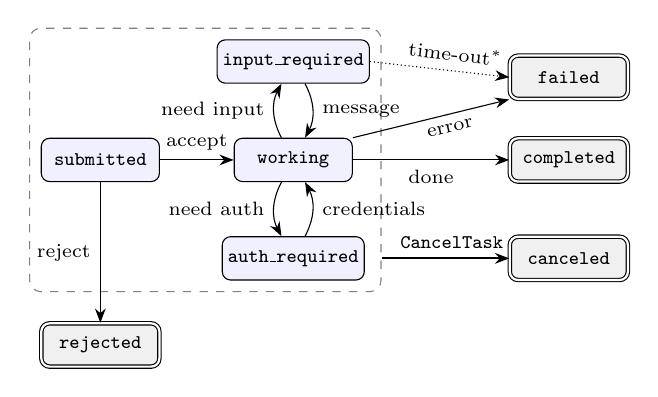
\begin{tikzpicture}[font=\scriptsize, >={Stealth[length=1.8mm]},
  st/.style={draw, rounded corners=3pt, fill=blue!6, minimum width=1.5cm,
    minimum height=0.55cm, inner sep=2pt},
  term/.style={st, fill=gray!12, double, double distance=0.8pt}]
\node[st] (sub) at (0,0) {\code{submitted}};
\node[st] (wrk) at (2.45,0) {\code{working}};
\node[st] (inp) at (2.45,1.25) {\code{input\_required}};
\node[st] (aut) at (2.45,-1.25) {\code{auth\_required}};
\node[term] (rej) at (0,-2.35) {\code{rejected}};
\node[term] (fai) at (5.95,1.05) {\code{failed}};
\node[term] (com) at (5.95,0) {\code{completed}};
\node[term] (can) at (5.95,-1.25) {\code{canceled}};
\begin{scope}[on background layer]
  \node[draw, dashed, gray, rounded corners=4pt, fit=(sub)(wrk)(inp)(aut),
    inner sep=4pt] (live) {};
\end{scope}
\draw[->] (sub) -- node[above]{accept} (wrk);
\draw[->] (sub) -- node[left]{reject} (rej);
\draw[->] (wrk) to[bend left=28] node[left]{need input} (inp);
\draw[->] (inp) to[bend left=28] node[right]{message} (wrk);
\draw[->] (wrk) to[bend right=28] node[left]{need auth} (aut);
\draw[->] (aut) to[bend right=28] node[right]{credentials} (wrk);
\draw[->] (wrk) -- node[below]{done} (com);
\draw[->] (wrk.north east) -- node[below, sloped, pos=0.6]{error} (fai.south west);
\draw[->, densely dotted] (inp.east) -- node[above, sloped, pos=0.6]{time-out$^{*}$} (fai.west);
\draw[->, thick] (live.east |- can) -- node[above, pos=0.55]{\code{CancelTask}} (can);
\end{tikzpicture}
\caption{A2A~v1.0 task lifecycle as realized by Listing~\ref{lst:fsm}.
Double borders mark terminal states, which the process reaches by journaling
the outcome and stopping normally. Cancellation is legal in every
non-terminal state (dashed region). $^{*}$The time-out on
\code{input\_required} is a deployment policy, not a protocol requirement.
\code{UNSPECIFIED} is never produced.}
\label{fig:fsm}
\end{figure}

\subsection{Shared Services}

The application supervisor also runs four shared services. The
\code{gateway} terminates A2A over HTTP, including server-sent events,
validates every message, decodes JSON into maps with binary keys, and never
creates atoms from input; conversion to atoms is limited to a fixed set
through \code{binary\_to\_existing\_atom/2}. The \code{registry} uses
\code{pg} process groups for local discovery and caches remote Agent Cards
only after their signatures have been verified. The \code{governor} enforces
token budgets, provider rate limits, and circuit breakers per provider and
model. Model-calling children consult it in their start functions, so a
restart attempt fails fast once the budget is exhausted; the supervisor
counts each failed attempt against its restart intensity and soon escalates.
This implements the budget-aware restart intensity examined in RQ3. The
\code{journal} stores checkpoints and the effect log in a durable database:
PostgreSQL across deployments, with Mnesia evaluated as an intra-domain
alternative.

\subsection{Non-Blocking Agents}

Listing~\ref{lst:async} shows the pattern that answers criticism C10. The
agent never blocks its mailbox on a model call: it records the caller,
returns immediately, and replies when the model client delivers the result.
Callers use \code{send\_request/2} with a time-out sized for model latency
rather than the 5{,}000\,ms default~\cite{otp-genserver}.

\begin{lstlisting}[float=t, caption={Deferred replies keep an agent's
mailbox responsive during slow model calls.}, label={lst:async}]
%% Server side: never block the mailbox.
handle_call({ask, Q}, From,
            S = #{pending := P}) ->
    Ref = model_client:request_async(Q),
    {noreply, S#{pending := P#{Ref => From}}}.

handle_info({model_reply, Ref, R},
            S = #{pending := P}) ->
    {From, P1} = maps:take(Ref, P),
    gen_server:reply(From, R),
    {noreply, S#{pending := P1}}.

%% Client side: explicit, model-sized time-out.
ask(Agent, Q) ->
    Id = gen_server:send_request(Agent, {ask, Q}),
    gen_server:receive_response(Id, 120000).
\end{lstlisting}

%% =====================================================================
\section{Methodology and Evaluation Plan}\label{sec:method}
%% =====================================================================

\subsection{Work Packages}

The work is organized into seven work packages; Appendix~\ref{app:plan}
gives their schedule and gates. WP0 is a systematic literature and artifact
review with a published protocol covering the ACM and IEEE digital
libraries, arXiv, the Erlang Workshop proceedings, Hex, and GitHub; it also
selects the durable-execution baseline. WP1 implements and verifies the
lifecycle machine against the TCK. WP2 builds the fault-injection harness
and a mock model server. WP3 builds the minimal prototype of
Fig.~\ref{fig:arch}. WP4 builds the baselines, WP5 runs the experiments,
and WP6 analyses and reports them. No general-purpose framework will be
built; the prototype contains only what the research questions require.

\subsection{Prototype}

The prototype will be written in Erlang on OTP~29~\cite{otp29} with rebar3,
using Cowboy for HTTP and server-sent events and OTP's built-in \code{json}
module. Remote Agent Cards will be verified with a JOSE library according to
the A2A~v1.0 signing rules~\cite{aaif2026}. Elixir is deliberately avoided
in the core so that the results speak to OTP rather than to any one
framework.

\subsection{Fault Model and Injection}\label{sec:faults}

Faults are injected at three layers. At the model layer, a deterministic
mock model server reproduces latency distributions fitted to measured
provider traces and injects HTTP~429 and 5xx responses, latency spikes,
truncated streams, malformed JSON, schema-violating structured output, and
scripted semantic errors whose wrongness an oracle can check. At the agent
layer, faults include process crashes, hangs (a process that stops
replying), runaway tool loops, and non-idempotent tool calls instrumented to
count their executions. At the infrastructure layer, faults include node
termination and network partitions, injected with
\code{erlang:disconnect\_node/1} for BEAM-internal partitions and with
operating-system traffic control for every configuration. Each fault is
injected before, during, and after a tool's effect, because that timing
determines whether a restart duplicates the effect.

\subsection{Workloads}

Two workload families are planned. Synthetic hierarchical tasks of depth one
to three and fan-out two to eight run against the mock model and allow
thousands of runs. A small case study, a research-assistant hierarchy over a
fixed document corpus, uses a locally served open-weight model to control
cost and model drift; hosted models are used only for a calibration subset.
Consistent with C13, all workloads are parallelizable by design.

\subsection{Metrics}

The primary metrics are task completion rate; time to detect and time to
recover from a failure (median and 99th percentile); wasted tokens, defined
as tokens spent on work that recovery later discards; duplicated side
effects; tokens consumed after \code{CancelTask}; and protocol violations
observed by an independent conformance monitor at the gateway. Secondary
metrics are runtime overhead excluding model time, memory per idle agent,
and implementation size, which is reported only with caution as a proxy for
effort.

\subsection{Baselines and Fairness}

B2 combines the official A2A Python SDK with LangGraph and a PostgreSQL
checkpointer~\cite{langgraph-durable}. B3 is a durable-execution runtime,
either Dapr Agents~\cite{dapr-agents} or Microsoft Agent
Framework~\cite{maf-vsm}, chosen in WP0 by maturity of A2A~v1.0 support. A
BEAM-internal baseline, Jido with persistence enabled~\cite{jido-storage},
separates the effect of the runtime from the effect of our design. To limit
implementer bias, baselines start from the vendors' own samples, are
reviewed by a practitioner fluent in each stack, and are released with all
other artifacts.

\subsection{Statistics and Pre-Registration}\label{sec:stats}

Mock-model experiments use at least 30 independent runs per configuration
and fault, while real-model runs use at least ten because of cost. Results
are reported as medians with bootstrap 95\% confidence intervals and
compared with Mann--Whitney $U$ tests under Holm--Bonferroni correction,
with Cliff's $\delta$ as the effect size. H2b uses non-inferiority tests
with margins fixed in advance. Hypotheses, margins, metrics, and analysis
code will be registered publicly, for example on the Open Science
Framework, before WP5 begins.

\subsection{Threats to Validity}

Internal validity is threatened by implementer bias and by the realism of
the mock model; the mitigations are external review of baselines and
calibration against real traces. External validity is limited by small
hierarchies and few workloads, a limitation we accept because of C13.
Construct validity is limited because wasted tokens are a proxy for cost and
code size is a proxy for effort. Conclusion validity is limited by multiple
comparisons, which the corrections address, and by low statistical power
for real-model runs, which we report.

%% =====================================================================
\section{Expected Outcomes and Go/No-Go Gates}\label{sec:gates}
%% =====================================================================

The project has three gates. At gate~G0, at the end of WP0, if a
peer-reviewed study already answers RQ2, RQ2 is dropped and the work
concentrates on RQ1 and RQ4. At gate~G1, at the end of WP1, if the lifecycle
machine cannot pass the mandatory TCK categories within its time box, claims
of A2A conformance are withdrawn and the experiments use an internal
protocol. At gate~G2, at the end of WP3, if checkpointing and effect
journaling cannot eliminate duplicated effects in the prototype, the project
reports why and stops before the performance comparisons.

The planned deliverables are a public dataset of fault-injection traces, the
open-source prototype and baselines, and a paper. Plausible venues include
the ACM SIGPLAN Erlang Workshop and workshops on actors and agents such as
the AGERE! series~\cite{agere}, subject to their calls at submission time.
The most likely outcome, stated in advance, is that the OTP design matches
durable-execution runtimes on recovery, beats checkpoint-only orchestration
on failure detection and cancellation, and shows no end-to-end performance
advantage. That outcome would still be publishable as a careful,
partly negative result, and it is the outcome against which success should
be judged.

%% =====================================================================
\section{Ethical, Security, and Cost Considerations}
%% =====================================================================

No experiment performs real side effects: every non-idempotent tool targets
an instrumented sandbox that stands in for e-mail, payment, or ticketing
services. Prompt-injection and poisoned-Agent-Card test cases come from
published threat models~\cite{habler2025,aaif2026} and are run only against
the project's own deployments. Vulnerabilities found in third-party
libraries, such as atom exhaustion from untrusted input, will be reported
through coordinated disclosure before publication. Spending on hosted models
is capped by the governor itself, and every experiment has a fixed budget
set before it runs.

%% =====================================================================
\section{Timeline and Feasibility}
%% =====================================================================

The plan spans eight months (Appendix~\ref{app:plan}). It is feasible for
one investigator only because of three scope decisions: no general-purpose
framework, shallow hierarchies, and mock models for the bulk of the runs.
The largest schedule risk is WP4, because building fair baselines in
unfamiliar stacks is slow; it is therefore started in parallel with WP3. The
risk register (Appendix~\ref{app:risk}) lists the remaining risks and their
mitigations.

%% =====================================================================
\section{Conclusion}
%% =====================================================================

Erlang/OTP looks made for A2A hierarchies, and that appearance is the
problem. The obvious mapping of agents to processes, teams to supervision
trees, and lifecycles to \gsm{} has been built many times, and it rests on
a fault model of fail-stop, transient, cheap-to-retry crashes that LLM
agents mostly violate. Supervisors do not see hallucinations, restarts
discard expensive context and can repeat side effects, restart intensity
becomes an unbudgeted spending policy, and distributed Erlang cannot cross
the organizational boundaries that A2A exists to cross. What remains is a
smaller and more honest research programme: supervise tasks rather than
agents, couple OTP's failure detection with durable state and an effect
journal, use \gsm{} to make the A2A lifecycle conformant by construction,
and measure, against strong baselines, whether this improves detection,
cancellation, and recovery cost. If it does not, that is worth knowing too.

%% =====================================================================
%% References (web sources accessed 18 Nov 2026)
%% =====================================================================
\begin{thebibliography}{99}
\footnotesize

\bibitem{hewitt1973}
C.~Hewitt, P.~Bishop, and R.~Steiger, ``A universal modular ACTOR formalism
for artificial intelligence,'' in \emph{Proc. 3rd Int. Joint Conf.
Artificial Intelligence (IJCAI)}, 1973, pp.~235--245.

\bibitem{agha1986}
G.~Agha, \emph{Actors: A Model of Concurrent Computation in Distributed
Systems}. Cambridge, MA, USA: MIT Press, 1986.

\bibitem{armstrong2003}
J.~Armstrong, ``Making reliable distributed systems in the presence of
software errors,'' Ph.D. dissertation, Royal Institute of Technology (KTH),
Stockholm, Sweden, 2003.

\bibitem{armstrong2007}
J.~Armstrong, ``A history of Erlang,'' in \emph{Proc. 3rd ACM SIGPLAN Conf.
History of Programming Languages (HOPL III)}, 2007, pp.~6-1--6-26.

\bibitem{cesarini2016}
F.~Cesarini and S.~Vinoski, \emph{Designing for Scalability with
Erlang/OTP}. Sebastopol, CA, USA: O'Reilly Media, 2016.

\bibitem{otp-sup}
Erlang/OTP, ``supervisor: Generic supervisor behavior,'' STDLIB Reference
Manual. [Online]. Available:
\url{https://www.erlang.org/doc/apps/stdlib/supervisor.html}

\bibitem{otp-sup-princ}
Erlang/OTP, ``Supervisor behaviour,'' OTP Design Principles. [Online].
Available: \url{https://www.erlang.org/doc/system/sup_princ.html}

\bibitem{otp-genserver}
Erlang/OTP, ``gen\_server: Generic server behavior,'' STDLIB Reference
Manual. [Online]. Available:
\url{https://www.erlang.org/doc/apps/stdlib/gen_server.html}

\bibitem{otp-statem}
Erlang/OTP, ``gen\_statem behaviour,'' OTP Design Principles. [Online].
Available: \url{https://www.erlang.org/doc/system/statem.html}

\bibitem{otp-dist}
Erlang/OTP, ``Distributed Erlang,'' Erlang System Documentation. [Online].
Available: \url{https://www.erlang.org/doc/system/distributed.html}

\bibitem{otp-limits}
Erlang/OTP, ``System limits,'' Erlang System Documentation. [Online].
Available: \url{https://www.erlang.org/doc/system/system_limits.html}

\bibitem{otp-eff}
Erlang/OTP, ``Advanced,'' Efficiency Guide, OTP~26. [Online]. Available:
\url{https://www.erlang.org/docs/26/efficiency_guide/advanced}

\bibitem{otp-nif}
Erlang/OTP, ``erl\_nif: API functions for an Erlang NIF library,'' ERTS
Reference Manual. [Online]. Available:
\url{https://www.erlang.org/doc/apps/erts/erl_nif.html}

\bibitem{otp29}
Erlang/OTP, ``Erlang/OTP 29.0,'' release announcement, May 13, 2026.
[Online]. Available: \url{https://www.erlang.org/news/188}

\bibitem{otp2902}
Erlang/OTP, ``Erlang/OTP 29.0.2,'' patch release notes, Jun. 10, 2026.
[Online]. Available: \url{https://www.erlang.org/patches/otp-29.0.2}

\bibitem{gray1985}
J.~Gray, ``Why do computers stop and what can be done about it?'' Tandem
Computers, Cupertino, CA, USA, Tech. Rep. 85.7, Jun. 1985.

\bibitem{candea2004}
G.~Candea, S.~Kawamoto, Y.~Fujiki, G.~Friedman, and A.~Fox,
``Microreboot---A technique for cheap recovery,'' in \emph{Proc. 6th USENIX
Symp. Operating Systems Design and Implementation (OSDI)}, 2004,
pp.~31--44.

\bibitem{trinder2017}
P.~Trinder \emph{et al.}, ``Scaling reliably: Improving the scalability of
the Erlang distributed actor platform,'' \emph{ACM Trans. Program. Lang.
Syst.}, vol.~39, no.~4, Art.~17, 2017, doi: 10.1145/3107937.

\bibitem{meiklejohn2019}
C.~S. Meiklejohn, H.~Miller, and P.~Alvaro, ``PARTISAN: Scaling the
distributed actor runtime,'' in \emph{Proc. USENIX Annual Technical Conf.
(ATC)}, 2019, pp.~63--76.

\bibitem{fowler2016}
S.~Fowler, ``An Erlang implementation of multiparty session actors,'' in
\emph{Proc. 9th Interaction and Concurrency Experience (ICE)}, EPTCS,
vol.~223, 2016, arXiv:1608.03321.

\bibitem{fowler2026}
S.~Fowler and R.~Hu, ``Speak now: Safe actor programming with multiparty
session types,'' arXiv:2602.24054, Feb. 2026.

\bibitem{distefano2003}
A.~Di~Stefano and C.~Santoro, ``eXAT: An experimental tool for programming
multi-agent systems in Erlang,'' in \emph{Proc. AI*IA/TABOO Joint Workshop
on Objects and Agents (WOA)}, Villasimius, Italy, 2003.

\bibitem{distefano2004}
A.~Di~Stefano and C.~Santoro, ``Designing collaborative agents with eXAT,''
in \emph{Proc. 13th IEEE Int. Workshops on Enabling Technologies:
Infrastructure for Collaborative Enterprises (WETICE)}, 2004, pp.~15--20.

\bibitem{distefano2005}
A.~Di~Stefano and C.~Santoro, ``Using the Erlang language for multi-agent
systems implementation,'' in \emph{Proc. IEEE/WIC/ACM Int. Conf. Intelligent
Agent Technology (IAT)}, 2005, pp.~679--685.

\bibitem{fernandez2013}
\'{A}.~Fern\'{a}ndez D\'{\i}az, C.~Benac Earle, and L.-\AA.~Fredlund,
``eJason: An implementation of Jason in Erlang,'' in \emph{Programming
Multi-Agent Systems (ProMAS 2012)}, ser. LNCS, vol.~7837. Berlin, Germany:
Springer, 2013, pp.~1--16, doi: 10.1007/978-3-642-38700-5\_1.

\bibitem{benacearle2017}
C.~Benac Earle, ``Building distributed and robust multi-agent systems,''
talk, Erlang User Conference, Stockholm, Sweden, 2017. [Online]. Available:
\url{https://www.erlang-factory.com/euc2017/clara-benac-earle}

\bibitem{a2a-spec}
A2A Project, ``Agent2Agent (A2A) protocol specification, version 1.0,''
2026. [Online]. Available:
\url{https://a2a-protocol.org/latest/specification/}

\bibitem{a2a-github}
A2A Project, ``a2aproject/A2A: Agent2Agent protocol,'' GitHub repository.
[Online]. Available: \url{https://github.com/a2aproject/A2A}

\bibitem{lf2025}
The Linux Foundation, ``Linux Foundation launches the Agent2Agent Protocol
Project to enable secure, intelligent communication between AI agents,''
press release, Jun. 23, 2025. [Online]. Available:
\url{https://www.linuxfoundation.org/press/linux-foundation-launches-the-agent2agent-protocol-project-to-enable-secure-intelligent-communication-between-ai-agents}

\bibitem{lf2026}
The Linux Foundation, ``A2A Protocol surpasses 150 organizations, lands in
major cloud platforms, and sees enterprise production use in first year,''
press release, Apr. 9, 2026.

\bibitem{axios2026}
Axios, ``Exclusive: Google-backed agentic A2A protocol gets a new home,''
Aug. 17, 2026. [Online]. Available:
\url{https://axios.com/2026/08/17/a2a-agentic-ai-foundation-open-ai-standards}

\bibitem{aaif2026}
Agentic AI Foundation, ``A2A v1.0: A builder's guide, part 2: Migration,
security, and production,'' 2026. [Online]. Available:
\url{https://aaif.io/blog/a2a-v1-0-a-builder-s-guide-part-2-migration-security-and-production}

\bibitem{habler2025}
I.~Habler, K.~Huang, V.~S. Narajala, and P.~Kulkarni, ``Building a secure
agentic AI application leveraging A2A protocol,'' arXiv:2504.16902, 2025.

\bibitem{cemri2025}
M.~Cemri \emph{et al.}, ``Why do multi-agent LLM systems fail?'' in
\emph{Advances in Neural Information Processing Systems (NeurIPS)}, 2025,
arXiv:2503.13657.

\bibitem{kim2025}
Y.~Kim \emph{et al.}, ``Towards a science of scaling agent systems,''
arXiv:2512.08296, Dec. 2025.

\bibitem{anthropic2025}
Anthropic, ``How we built our multi-agent research system,'' Anthropic
Engineering, Jun. 2025. [Online]. Available:
\url{https://www.anthropic.com/engineering/multi-agent-research-system}

\bibitem{yan2025}
W.~Yan, ``Don't build multi-agents,'' Cognition, Jun. 12, 2025. [Online].
Available: \url{https://cognition.ai/blog/dont-build-multi-agents}

\bibitem{yan2026}
W.~Yan, ``Multi-agents: What's actually working,'' Cognition, Apr. 22,
2026. [Online]. Available:
\url{https://cognition.ai/blog/multi-agents-working}

\bibitem{autogen2025}
Microsoft Research, ``AutoGen v0.4: Reimagining the foundation of agentic AI
for scale, extensibility, and robustness,'' Microsoft Research Blog, Jan.
2025.

\bibitem{maf-sdtimes}
SD Times, ``Microsoft announces preview of its new Agent Framework,'' Oct.
2025. [Online]. Available:
\url{https://sdtimes.com/msft/microsoft-announces-preview-of-its-new-agent-framework/}

\bibitem{maf-vsm}
Visual Studio Magazine, ``Microsoft ships production-ready Agent Framework
1.0 for .NET and Python,'' Apr. 6, 2026.

\bibitem{gao2024}
D.~Gao \emph{et al.}, ``AgentScope: A flexible yet robust multi-agent
platform,'' arXiv:2402.14034, 2024.

\bibitem{akka2025}
Akka, ``Announcing the Akka Agentic Platform,'' Jul. 2025. [Online].
Available: \url{https://akka.io/blog/announcing-akkas-agentic-ai-release}

\bibitem{akka-capabilities}
Akka, ``Agentic AI platform capabilities reference.'' [Online]. Available:
\url{https://akka.io/platform/capabilities}

\bibitem{akka-patterns}
Akka, ``AI orchestration patterns,'' Akka documentation. [Online].
Available: \url{https://doc.akka.io/concepts/ms-agent-patterns.html}

\bibitem{dapr-agents}
Dapr Project, ``Dapr Agents: A framework for agentic AI systems,'' PyPI
package \code{dapr-agents} 1.0.1. [Online]. Available:
\url{https://pypi.org/project/dapr-agents/}

\bibitem{dapr-docs}
Dapr Project, ``Overview,'' Dapr documentation. [Online]. Available:
\url{https://docs.dapr.io/overview/}

\bibitem{cloudflare-agents}
Cloudflare, ``Agent class,'' Cloudflare Agents documentation. [Online].
Available:
\url{https://developers.cloudflare.com/agents/runtime/lifecycle/agent-class/}

\bibitem{langgraph-durable}
LangChain, ``Durable execution,'' LangGraph documentation. [Online].
Available: \url{https://docs.langchain.com/oss/python/langgraph/durable-execution}

\bibitem{diagrid2025}
Diagrid, ``Checkpoints are not durable execution: Why LangGraph, CrewAI,
Google ADK and others fall short for production agent workflows,'' vendor
blog. [Online]. Available:
\url{https://www.diagrid.io/blog/checkpoints-are-not-durable-execution-why-langgraph-crewai-google-adk-and-others-fall-short-for-production-agent-workflows}

\bibitem{adk-multi}
Google, ``Multi-agent systems in ADK,'' Agent Development Kit documentation.
[Online]. Available: \url{https://google.github.io/adk-docs/agents/multi-agents/}

\bibitem{jido}
Agent Jido, ``jido: Autonomous agent framework for Elixir,'' GitHub
repository. [Online]. Available: \url{https://github.com/agentjido/jido}

\bibitem{jido-storage}
Agent Jido, ``Persistence \& storage,'' Jido documentation. [Online].
Available: \url{https://hexdocs.pm/jido/storage.html}

\bibitem{langchain-ex}
M.~Ericksen \emph{et al.}, ``Elixir LangChain,'' GitHub repository.
[Online]. Available: \url{https://github.com/brainlid/langchain}

\bibitem{sagents}
Sagents, ``sagents: Interactive AI agents in Elixir with OTP supervision,''
GitHub repository. [Online]. Available:
\url{https://github.com/sagents-ai/sagents}

\bibitem{sagents-readme}
Sagents, ``README, version 0.8.0,'' Hex package documentation. [Online].
Available: \url{https://readme.hex.pm/sagents/0.8.0}

\bibitem{exagent}
``exagent: A layered agent framework for Elixir,'' Hex package. [Online].
Available: \url{https://hex.pm/packages/exagent}

\bibitem{condukt}
``Condukt: A framework for building AI agents in Elixir,'' Hex package
README. [Online]. Available: \url{https://readme.hex.pm/condukt/0.9.0}

\bibitem{lux}
Spectral Finance, ``Lux: A framework for building and orchestrating
LLM-powered agent workflows,'' GitHub repository. [Online]. Available:
\url{https://github.com/Spectral-Finance/lux}

\bibitem{erlang-adk}
``Erlang ADK (Agent Development Kit),'' Hex package README, version 0.9.0.
[Online]. Available: \url{https://readme.hex.pm/erlang_adk/0.9.0}

\bibitem{erlangchain}
``erlangchain: Minimal building blocks for talking to LLMs from Erlang,''
Hex package README. [Online]. Available:
\url{https://readme.hex.pm/erlangchain/0.4.0}

\bibitem{a2a-actioncard}
ActionCard, ``a2a: Elixir implementation of the Agent-to-Agent (A2A)
protocol,'' GitHub repository and Hex package. [Online]. Available:
\url{https://github.com/actioncard/a2a-elixir}

\bibitem{a2a-ex}
``a2a\_ex: Elixir client and server library for the Agent2Agent protocol,''
Hex package documentation. [Online]. Available:
\url{https://hexdocs.pm/a2a_ex/readme.html}

\bibitem{a2a-engine}
``A2aEngine: Pure-spec implementation of the Agent2Agent protocol,'' Hex
package README, version 0.1.0. [Online]. Available:
\url{https://readme.hex.pm/a2a_engine/0.1.0}

\bibitem{a2a-elixir-sdk}
``A2AEx: Elixir implementation of the Agent-to-Agent protocol,'' Hex package
\code{a2a\_elixir\_sdk}, version 1.0.1. [Online]. Available:
\url{https://readme.hex.pm/a2a_elixir_sdk/1.0.1}

\bibitem{cve2025-32433}
F.~B\"{a}umer, M.~Brinkmann, M.~Maehren, and J.~Schwenk, ``CVE-2025-32433:
Unauthenticated remote code execution in Erlang/OTP SSH,'' oss-security
mailing list, Apr. 16, 2025. [Online]. Available:
\url{https://seclists.org/oss-sec/2025/q2/52}

\bibitem{cve2025-32433-kev}
CIRCL Vulnerability-Lookup, ``CVE-2025-32433,'' record including the CISA
Known Exploited Vulnerabilities entry of Jun. 9, 2025. [Online]. Available:
\url{https://cve.circl.lu/cve/CVE-2025-32433}

\bibitem{cve2026-48860}
SentinelOne, ``CVE-2026-48860: Erlang/OTP \code{inet\_tls\_dist}
authorization bypass,'' vulnerability database entry. [Online]. Available:
\url{https://www.sentinelone.com/vulnerability-database/cve-2026-48860/}

\bibitem{agere}
A.~Ricci, G.~Agha, R.~H. Bordini, and A.~Marron, ``Special issue on
programming based on actors, agents and decentralized control,''
\emph{Sci. Comput. Program.}, vol.~98, pt.~2, 2015.

\end{thebibliography}

%% =====================================================================
%% Appendices follow the references and are typeset in one column so that
%% each table sits next to its text.
\onecolumn
\appendices
%% =====================================================================

\section{Comparison of Existing Solutions}\label{app:matrix}

Table~\ref{tab:matrix} summarizes the survey of Section~\ref{sec:survey}.
Entries reflect public documentation consulted in November 2026; ``n/r''
means \emph{not reported in the sources we consulted}, which is absence of
evidence rather than evidence of absence.

\begin{table}[!h]
\centering
\caption{Existing solutions related to Erlang/OTP-based A2A hierarchies}
\label{tab:matrix}
\footnotesize
\renewcommand{\arraystretch}{1.12}
\begin{tabularx}{\textwidth}{@{}P{2.9cm}P{1.6cm}YYYP{2.3cm}P{1.9cm}@{}}
\toprule
\textbf{System} & \textbf{Platform} & \textbf{Agents as processes or actors}
 & \textbf{Failure handling} & \textbf{Durable agent state}
 & \textbf{A2A support} & \textbf{Status} \\
\midrule
eXAT~\cite{distefano2003,distefano2004} & Erlang & Yes; FSM behaviours
 & n/r & No & No (FIPA-ACL) & Prototype, 2003--05 \\
eJason~\cite{fernandez2013,benacearle2017} & Erlang & Yes; agent = process
 & Erlang-inspired monitoring & No & No & Research prototype \\
Jido 2.x~\cite{jido,jido-storage} & Elixir & Yes; \gs-based runtime,
 parent--child hierarchies & OTP supervision & Yes (hibernate/thaw) & n/r
 & Active open source \\
Sagents~\cite{sagents,sagents-readme} & Elixir & Yes; supervised \gs{}
 per agent & OTP supervision & Yes; optional cluster migration & n/r
 & Active open source \\
ExAgent~\cite{exagent} & Elixir & Yes; supervised process per agent
 & OTP supervision & Yes (pluggable stores) & n/r & Active open source \\
Lux~\cite{lux} & Elixir, Python & Yes & OTP supervisor & n/r & n/r
 & Open source \\
Condukt~\cite{condukt} & Elixir & Yes & OTP supervision trees & n/r & n/r
 & Open source \\
Erlang ADK~\cite{erlang-adk} & Erlang & n/r & n/r & Session data & n/r
 & Early (0.9) \\
\code{a2a}~\cite{a2a-actioncard} & Elixir & Yes; \gs{} per agent
 & Agent supervisor & ETS by default, pluggable & Yes (0.3, 1.0; TCK)
 & Pre-release \\
\code{a2a\_ex}~\cite{a2a-ex} & Elixir & n/a (codec, transport) & n/a
 & ETS adapter & Yes (0.3) & Early \\
\code{a2a\_engine}~\cite{a2a-engine} & Elixir & n/a (spec, codecs)
 & n/a & Host-owned & Yes; pluggable transport & Early \\
\code{a2a\_elixir\_sdk}~\cite{a2a-elixir-sdk} & Elixir & Bridges agent kit
 & n/r & In-memory stores & Yes (JSON-RPC, SSE) & 1.0.1 \\
AutoGen 0.4 / MS Agent Framework~\cite{autogen2025,maf-sdtimes,maf-vsm}
 & Python, .NET & Yes (AutoGen Core) & n/r & n/r & Yes (Agent Framework)
 & 1.0, Apr.~2026 \\
AgentScope~\cite{gao2024} & Python & Yes; actor-based distribution
 & Built-in fault tolerance for LLM and API errors & n/r & n/r
 & Research platform \\
Akka Agentic Platform~\cite{akka2025,akka-capabilities,akka-patterns}
 & JVM & Yes; agents do not spawn sub-agents & Parent supervision, backoff
 & Yes (durable memory) & n/r & Commercial \\
Dapr Agents~\cite{dapr-agents,dapr-docs} & Python + Dapr & Yes; workflows
 on virtual actors & Durable-execution recovery & Yes & n/r & 1.0.x \\
Cloudflare Agents~\cite{cloudflare-agents} & TypeScript & Yes; Durable
 Objects & Platform-managed & Yes (per-agent storage) & n/r & Vendor SDK \\
LangGraph~\cite{langgraph-durable,diagrid2025} & Python, JS & No (graph
 nodes) & Resume from checkpoint; detection external & Yes (checkpointer)
 & n/r & Mature \\
Google ADK~\cite{adk-multi} & Python and others & Parent/sub-agent tree
 & n/r & n/r & n/r & Mature \\
\midrule
\textbf{This proposal} & Erlang/OTP 29 & Yes; task-tree supervision
 & OTP supervision, budget-aware restarts, effect journal & Yes (journal)
 & Yes (1.0; TCK) & Proposed \\
\bottomrule
\end{tabularx}
\end{table}

\clearpage
\section{Mapping of A2A Task States to OTP Mechanisms}\label{app:map}

Table~\ref{tab:map} complements Fig.~\ref{fig:fsm} and
Listing~\ref{lst:fsm}.

\begin{table}[!h]
\centering
\caption{A2A v1.0 task states and their realization}
\label{tab:map}
\footnotesize
\renewcommand{\arraystretch}{1.12}
\begin{tabularx}{\textwidth}{@{}P{3.0cm}P{2.0cm}Y@{}}
\toprule
\textbf{TaskState} & \textbf{Category} & \textbf{Realization in OTP} \\
\midrule
\code{SUBMITTED} & live & Initial state; enter call journals \\
\code{WORKING} & live & Agent loop running; follow-up messages postponed \\
\code{INPUT\_REQUIRED} & interrupted & Waits for client message;
 \code{state\_timeout} (policy) \\
\code{AUTH\_REQUIRED} & interrupted & Waits for out-of-band credentials;
 never reused across interruptions \\
\code{COMPLETED} & terminal & Journal, stop \code{normal};
 \code{auto\_shutdown} of subtree \\
\code{FAILED} & terminal & As above; also reported by the gateway when a
 subtree disappears without a terminal record (e.g., exhausted restart
 intensity) \\
\code{CANCELED} & terminal & Journal \code{CANCELED} for self and live
 descendants, reply, stop; subtree shutdown reclaims processes;
 \code{a2a\_client} children cancel remote peers in \code{terminate/2} \\
\code{REJECTED} & terminal & Reachable from \code{SUBMITTED} only \\
\code{UNSPECIFIED} & --- & Never produced; rejected by the gateway \\
\bottomrule
\end{tabularx}
\end{table}

\section{Risk Register}\label{app:risk}

Table~\ref{tab:risk} lists the principal risks with their likelihood (L)
and impact (I) rated low, medium, or high.

\begin{table}[!h]
\centering
\caption{Risk register}
\label{tab:risk}
\footnotesize
\renewcommand{\arraystretch}{1.12}
\begin{tabularx}{\textwidth}{@{}P{5.2cm}ccY@{}}
\toprule
\textbf{Risk} & \textbf{L} & \textbf{I} & \textbf{Mitigation} \\
\midrule
Prior work already answers RQ2 & M & H & WP0 first; pivot at G0 \\
Weak baselines (implementer bias) & H & H & Vendor samples; external
 review; open artifacts \\
Unrealistic mock model & M & M & Calibrate on real traces; real-model
 case study \\
Model drift or retirement & H & M & Pin versions; local open-weight model;
 archive traces \\
Spending overrun & M & M & Governor hard cap; mock-first design \\
Specification churn (v1.1) & M & M & Target v1.0.x; version negotiation;
 report TCK version \\
Immature community libraries & M & L & Own minimal stack; pinned
 dependencies \\
Null results throughout & M & M & Pre-registration; negative-result
 framing \\
Scope creep into a framework & H & H & Time-boxed WP3; no general API \\
\bottomrule
\end{tabularx}
\end{table}

\section{Work Plan}\label{app:plan}

\begin{table}[!h]
\centering
\caption{Work packages, schedule, and gates (months 1--8)}
\label{tab:plan}
\footnotesize
\renewcommand{\arraystretch}{1.12}
\begin{tabularx}{\textwidth}{@{}P{1.0cm}P{1.4cm}YP{1.0cm}@{}}
\toprule
\textbf{WP} & \textbf{Months} & \textbf{Output} & \textbf{Gate} \\
\midrule
WP0 & 1 & Review protocol and results; pre-registration draft & G0 \\
WP1 & 2--3 & Lifecycle machine; TCK report; fuzzing results & G1 \\
WP2 & 2--4 & Fault-injection harness; calibrated mock model & --- \\
WP3 & 3--5 & Minimal prototype with journal and governor & G2 \\
WP4 & 3--6 & Baselines B2, B3, and Jido, externally reviewed & --- \\
WP5 & 6--7 & Experiments for RQ1--RQ5; trace dataset & --- \\
WP6 & 7--8 & Analysis; paper; artifact release & --- \\
\bottomrule
\end{tabularx}
\end{table}

\end{document}
